\chapter{Probability theory}
\label{cha:probability}

\section{Discrete random variables}
A discrete variable can assume a value in a range of possible values, it can not
get values in between.

\defi{\textbf{Probability mass function}: \label{defi_prob_mass_funct}\\ Given a discrete random variable $X$ taking values in $\mathcal{X}= \{v_{1}, ..., v_{n}\}$, its probability mass function $P: \mathcal{X}\rightarrow [0, 1]$ is defined as: \[P(V_{i}) = Pr(X=v_{i})\] and satisfies the following conditions: \begin{itemize}\item $P(x) \geq 0$

\item $\sum_{x \in \mathcal{X}}{P(x)}= 1$\end{itemize} }

\defi{\textbf{Expected value}: \label{def:expected_value}\\ The expected value (mean or average) of a random variable is: \[E[X] = \mu = \sum_{x \in \mathcal{X}}xP(x) = \sum_{i=1}^{m}v_{i}P(v_{i})\] This is a linear operator, that implies: \[E[\lambda x +\lambda ' y] = \lambda E[y] + \lambda ' E[y]\] }

\defi{\textbf{Variance}: \label{def:variance}\\ The variance of a random variable is the moment of inertia of its probability mass function: \[Var[x] = \sigma^{2}= E[(x - \mu)^{2}] = \sum_{x \in \mathcal{X}}(x - \mu)^{2}P(x)\] The standard deviation $\sigma$ indicates the typical amount of deviation from the mean one should expect for a randomly drawn value of x. }

Variance is \textbf{not} a linear operator. Therefore:\\
\[
	Var[x] = E[x^{2}] = E[x]^{2}
\]
\[
	Var[\lambda x] = \lambda^{2}Var[X]
\]
And for \textbf{uncorrelated variables} $x, y$ it is true that\\
\[
	Var[x+y] = Var[x] + Var[y]
\]

\subsection{Probability distributions for discrete variables}

\defi{\textbf{Bernoulli distribution}: \label{defi:bernoullo_dist}\\ The Bernoulli distribution applies on variables that can assume binary outcomes (0/1, true/false, success/failure). Being $p$ the parameter of success, its probability mass function is defines as: \[P(x;p) = \begin{cases}p&if\ x = 1\\ 1-p&if\ x = 0\end{cases}\] The expected value for a Bernoulli distribution is $p$ and the variance is equal to $p(1-p)$. }

\defi{\textbf{Binomial distribution}: \label{def:binomial_dist}\\ The binomial distribution is a Bernoulli distribution extended to a certain number $n$ of trials. Its probability mass function is: \[P(x;p,n) = \binom{n}{x}p^{x}(1-p)^{n-x}\] The expected value for a Binomial distribution is $np$ and the variance is equal to $np(1-p)$. }

It is easy to see that a Bernoulli distribution is per se a Binomial distribution
in the trivial case where $n=1$.\\ A Bernoulli distribution can be used for modelling
the toss of a coin, whereas the Binomial distribution describes the event of the
coin has been tossed $n$ times.

\defi{\textbf{Multinomial distribution}\label{def:mutltinomial_dist}\\ The multinomial distribution models the probability of an event that can have $m$ different outcomes, each with (possibly) a different probability. Its probability mass function is: \[P(x_{1}, \dots, x_{m}; p_{1}, \dots p_{m}) = \prod_{i=1}^{m}p_{i}^{x_i}\] where \begin{itemize}\item $x_{1}, \dots, x_{m}$ is a vector that represents the outcome,

\item $E[x_{i}] = p_{i}$

\item $Var[x_{i}] = p_{i}(1-p_{i})$

\item $Cov[x_{i}, x_{j}] = -p_{i}p_{j}$\end{itemize} }

Examples of outcome vectors for a 6-faces dice (d6) are:
\[
	x_{1}= [1, 0, 0, 0, 0, 0],
\]
\[
	x_{2}= [0, 1, 0, 0, 0, 0],
\]
\[
	x_{3}= [0, 0, 1, 0, 0, 0],
\]
\[
	x_{4}= [0, 0, 0, 1, 0, 0],
\]
\[
	x_{5}= [0, 0, 0, 0, 1, 0],
\]
\[
	x_{6}= [0, 0, 0, 0, 0, 1]
\]
in which the first column represents the success of the event of getting one as result,
the second column the event of getting two and so on so forth. Since the event are
mutually exclusive, just one column is signed as $1$. For a fair dice, the
vector or probabilities would be:
\[
	p = \left[ \frac{1}{6}, \frac{1}{6}, \frac{1}{6}, \frac{1}{6}, \frac{1}{6}, \frac{1}{6}
	\right]
\]

\defi{\textbf{Multinomial distribution (general case)}\\ Given $n$ repetition of an event which can end in $m$ possible outcome, $p=\{p_{1}, \dots, p_{m}\}$ the probability of each of the outcomes, the probability mass function is \[P(x_{1}, \dots, x_{m}; p_{1}, \dots, p_{m}, n) = \dfrac{n!}{\prod\limits_{i=1}^mx_i!}\prod\limits_{i=1}^{m}p_{i}^{x_i}\] In this distribution $E[x_{i}] = np_{i}$, $Var[x_{i}] = np_{i}(1-p_{i})$ and $Cov[x_{i}, x_{j}] = -np_{i}p_{j}$ }
Also this last case is a generalization of every case described above, but four
our purposes will not be used, it is reported for completeness.

\subsection{Pairs of discrete random variables}

\defi{\textbf{Joint probability mass function}: \label{def:joint_prob_mass_funct}\\ Given a pair of discrete random variables $X, Y$ taking values $\mathcal{X}= \{v_{1}, ..., v_{n}\}$ and $\mathcal{Y}= \{y_{1}, ..., y_{n}\}$, the joint probability mass function is defined as: \[P(v_{i}, w_{j}) = Pr[X = v_{i}, Y = w_{j}]\] This function has the following properties: \begin{itemize}\item $P(x, y) \geq 0$

\item $\sum_{x \in \mathcal{X}}\sum_{y \in \mathcal{Y}}P(x, y) = 1$\end{itemize} }

Its expected values are:
\[
	\mu_{x}= E[x] = x\sum_{x \in \mathcal{X}}\sum_{y \in \mathcal{Y}}P(x, y)
\]
\[
	\mu_{y}= E[y] = y\sum_{x \in \mathcal{X}}\sum_{y \in \mathcal{Y}}P(x, y)
\]
The variances are:
\[
	\sigma_{x}^{2}= Var[(x - \mu_{x})^{2}] = \sum_{x \in \mathcal{X}}\sum_{y \in
	\mathcal{Y}}(x - \mu_{x})^{2}P(x, y)
\]
\[
	\sigma_{y}^{2}= Var[(y - \mu_{y})^{2}] = \sum_{x \in \mathcal{X}}\sum_{y \in
	\mathcal{Y}}(y - \mu_{y})^{2}P(x, y)
\]
The covariance (expectation of how much they can co-vary) is:
\[
	\sigma_{xy}= E[(x-\mu_{x})(y-\mu_{y})] = \sum_{x\in \mathcal{X}}\sum_{y \in
	\mathcal{Y}}(x-\mu_{x}) (y - \mu_{y}) P(x, y)
\]
From these values we can get a coefficient of correlation as:
\[
	\rho = \frac{\sigma_{xy}}{\sigma{x}\sigma{y}}
\]
This measure is the ratio between the covariance of two variables and the
product of their standard deviations; thus, it is essentially a normalized
measurement of the covariance, such that the result always has a value between -1
and 1.

\section{Conditional probabilities}
If two variables are not independent, we can apply some laws and rules to get
their probability and conditional probabilities.

\theo{\textbf{Law of total probability}\\ The marginal distribution of a variable is obtained from a joint distribution summing over all possible values of the other variable.

\[P(x) = \sum_{y \in \mathcal{Y}}P(x, y)\] and \[P(y) = \sum_{x \in \mathcal{X}}P(x, y)\] }

\theo{\textbf{Produt rule, Bayes' rule}\label{theo:bayes}\\ Given two variables $x, y$ we can get the conditional probability from Bayes' rule as: \[P(x|y)P(y) = p(y|x)P(x)\] }

This is important because it allows to get information about a posterior
probability given the initial conditions and the likelihood of the linkage.

\[
	posterior = \frac{likelihood \times prior}{evidence}
\]

Prior and evidence are the data related to the single variables and likelihood is
the effect produced by the cause.\\ These rules apply also to more than two variables:
\[
	P(y) = \sum_{x}\sum_{z}P(x, y, z)
\]
\[
	P(y) = \sum_{x}\sum_{z}P(y | x, z) P(x, z)
\]
also for conditional probability:
\[
	P(y) = \sum_{x}\sum_{y}\frac{P(x|y, x)P(y|z)P(x, z)}{P(x|z)}
\]
Overall it is true that:
\[
	P(y|x, z) = \frac{P(x|z, y)P(y|z)}{P(x|z)}
\]

\section{Continuous random variables}
Continuous variables allows us to assign non-discrete values, for example the
height of a range of people, what we do is assigning intervals. The probability
mass function can be generalized on continuous domains.\\ Given
$W = (a < X \leq b)$ then $A = (X \leq a)$ and $B = (X \leq b)$. W and A end up to
be mutually exclusive, so
\[
	P(B) = P(A) + P(W)
\]

\defi{\textbf{Cumulative distribution}\label{def:cumulative_dist}\\ Given a continuous variable $X$ we define \[F(q) = P(X \leq q)\] the cumulative distribution of X. F is a monotonic function.\\ Given and interval $a < X \leq b$, the probability of $X$ is described as the difference of the edge values: \[P(a < X \leq b) = F(b) - F(a)\] }

\defi{\textbf{Probability density function}\label{def:prob_density_func}\\ The derivative of the cumulative distribution is called density function. \[p(x) = \frac{d}{dx}F(x)\] This corresponds to the mass function for continuous values. Therefore is true that \[F(q) = P(X \leq q) = \int_{-\infty}^{q}p(x)dx\] The probability density function has these properties: \begin{itemize}\item $p(x) \geq 0$

\item $\int_{-\infty}^{\infty}p(x)dx = 1$ which stands for the sum of all possible cases.\end{itemize} }

Also mean and variance \ref{def:expected_value} \ref{def:variance} are computed in
the same way, but taking into account the infinite number of small interval, therefore
computing an integral as well.

\[
	E[x] = \mu = \int_{-\infty}^{\infty}xp(x)dx
\]
\[
	Var[x] = \sigma^{2}= \int_{-\infty}^{\infty}(x-\mu)^{2}p(x)dx
\]

\subsection{Probability distributions for continuous variables}
\defi{\textbf{Gaussian or Normal distribution ($\mathcal{N}$)}\label{def:gaussian_normal}\\ The Gaussian distribution is a bell-shaped function that is the standard for fitting continuous data. The mean is the highest point in the graph while the variance is the spreading of the data from the mean.\\ The probability density function is \[p(x; \mu, \sigma) = \frac{1}{\sqrt{2\pi}\sigma}\exp^{-\frac{(x-\mu)^{2}}{2\sigma^{2}}}\] A standard distribution is denoted as $\mathcal{N}(0, 1)$ where $\mu = 0$ and $\sigma = 1$, \\ whereas a standardization of a normal distribution is $\mathcal{N}(\mu, \sigma^{2})$, it is carried on through this formula: \[z = \frac{x-\mu}{\sigma}\] }

\begin{center}
	\begin{figure}[H]
		\centering
		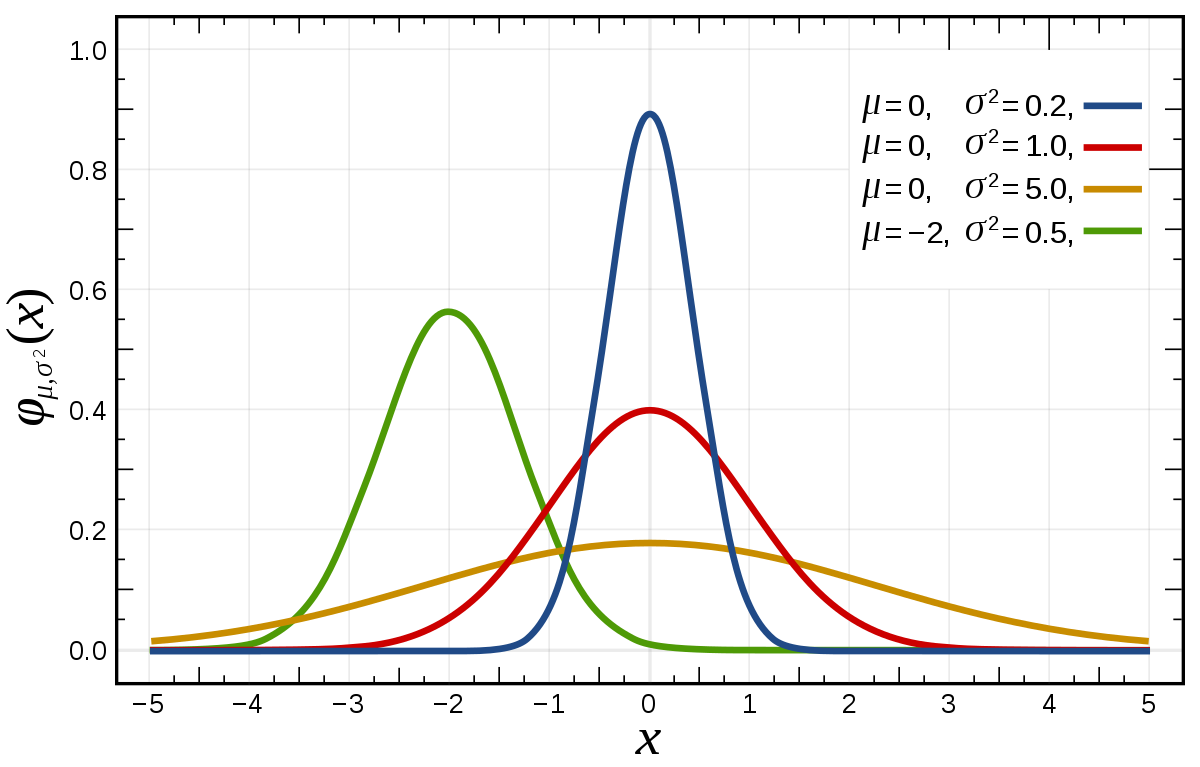
\includegraphics[scale=0.25]{images/05_ProbabilityTheory_gaussian.png}
		\caption{Set of Gaussian distributions}
		\label{fig:Gaussian_1}
	\end{figure}
\end{center}

\defi{\textbf{Beta distribution}\label{def:beta_dist}\\ The beta distribution is a second degree order of probability distribution (as the probability of a probability) that is defined in the interval $[0, 1]$ with parameters $\alpha$ and $\beta$. Its probability density function is \[p(x;\alpha, \beta) = \frac{\Gamma(\alpha + \beta)}{\Gamma(\alpha)\Gamma(\beta)}x^{\alpha-1}(1-x)^{\beta-1}\] where \begin{itemize}\item $\mathbb{E}[x] = \frac{\alpha}{\alpha+\beta}$

\item $Var[x] = \frac{\alpha\beta}{(\alpha+\beta)^{2}(\alpha+\beta+1)}$

\item $\Gamma(x+1) = x\Gamma(x)$

\item $\Gamma(1) = 1$\end{itemize} }
This distribution focuses on describing the distribution of a parameter $p$ of a
binomial distribution after observing $\alpha -1$ independent events with
probability $p$ and $\beta -1$ with probability $1-p$.

\defi{\textbf{Multivariate normal distribution}\label{def:multi_normal_dist}\\ This distribution aims to define a Gaussian distribution extended to $d$ dimensions. In order to define such distribution we need a mean $\mu$ and $\Sigma$ covariance matrix. Its probability density function is described as \[p(\vec{x}, \vec{\mu}, \Sigma) = \frac{1}{(2\pi)^{\frac{d}{2}}|\Sigma|^{\frac{1}{2}}}e^{-\frac{1}{2}(\vec{x}-\vec{\mu})^T\Sigma^{-1}(\vec{x}-\vec{\mu})}\] Relevant features are: \begin{itemize}\item $E[x] = \mu$

\item $Var[x] = \Sigma$

\item the squared Mahalanobis distance from x to $\mu$ is \\$r^{2}= (x-\mu)^{T}\Sigma^{-1}(x-\mu)$\end{itemize} }

\begin{figure}[H]
	\centering
	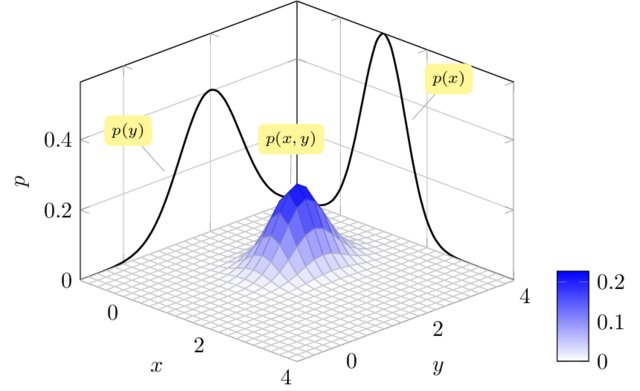
\includegraphics[scale=1]{
		images/05_ProbabilityTheory_multivariateDistribution.jpg
	}
	\caption{Multivariate normal distribution for $d=3$}
	\label{fig:Gaussian_2}
\end{figure}

\defi{\textbf{Dirichlet distribution}\label{def:diri_dist}\\ This distribution is defined for $x \in [0, 1]^{m}$, $\sum_{i=1}^{m}x_{i}= 1$, the parameters it is based on are $\alpha = \alpha_{1}, \dots, \alpha_{m}$ and its probability density function is \[p(x_{1}, \dots, x_{m}; \vec{\alpha}) = \frac{\Gamma(\alpha_{0})}{\prod\limits_{i=1}^{m}\Gamma(\alpha_{i})}\prod\limits_{i=1}^{m}x_{i}^{a_i-1}\] Where $\alpha_{0}= \sum_{j=1}^{m}\alpha_{j}$.

Characterizing values of this distribution are: \begin{itemize}\item $E[x_{i}] = \frac{\alpha_{1}}{\alpha_{0}}$

\item $Var[x_{i}] = \frac{\alpha_{i}(\alpha_{0}-\alpha_{i})}{\alpha_{0}^{2}(\alpha_{0}+1)}$

\item $Cov[x_{i}, x_{j}] = \frac{-\alpha_{i}\alpha_{j}}{a_{0}^{2}(\alpha_{0}+1)}$\end{itemize}

This distribution can model a posterior distribution of parameters $p$ of a multinomial distribution after observing $\alpha_{i}-1$ times each mutually exclusive events. }

\section{Probability laws}
Let's consider a sample of $X_{1}, \dots, X_{n}$ \textbf{independent} instances
from a distribution with mean $\mu$ and variance $\sigma^{2}$. We can get a \textbf{mean
of the obervated values} as
\[
	\bar{X}_{n}= \frac{X_{1}+ \dots + X_{n}}{n}
\]
and his expectation will be equals to $\mu$
\[
	E[\bar{X}_{n}] = \mu
\]
Its variance (iff they are \textbf{independent}) will be computed as
\[
	Var[a(X+Y)] = a^{2}(Var[X] + Var[Y])
\]
and the mean of the computed variance will be
\[
	Var[\bar{X}_{n}] = \frac{1}{n^{2}}(Var[X_{1}] + \cdots Var[X_{n}]) = \frac{\sigma^{2}}{n}
\]
that means that the variance of the average decreases as the number of observation
increases (the higher the number of the observation, the higher the precision of
the estimate).

\theo{\textbf{Chebyshev's inequality}\label{theo:Chebyshev}\\ Given a random variable $X$ with mean $\mu$ and variance $\sigma^{2}$, for all $a > 0$ \[Pr[|X-\mu| \geq a] \leq \frac{\sigma^{2}}{a^{2}}\] this implies the more $X$ differs from the mean more than $a$ the more $\sigma^{2}$ gets bigger and vice versa.\\ Also, replacing $a = k\sigma$ for $k>0$ \[Pr[|X - \mu| \geq k\sigma] \leq \frac{1}{k^{2}}\] This inequality shows that most of the probability mass of a random variable stays within few standard deviations from its mean. }

\theo{\textbf{Law of large numbers}\label{theo:large_numbers}\\ Considering a sample of $X_{1}, \dots, X_{n}$ independent instances from a distribution with mean $\mu$ and variance $\sigma^{2}$, for any $\epsilon > 0$ it is true that the object $\bar{X_n}$ obeys: \[\lim_{n \rightarrow \infty}Pr[|\bar{X_n}| > \epsilon] = 0\] Using Chebyschev's inequality and knowing that $E[\bar{X_n}] = \mu$ and also $Var[\bar{X_n}] = \frac{\sigma^{2}}{n}$ it comes that \[Pr[|\bar{X_n}- E[\bar{X_n}]| > \epsilon] \leq \frac{\sigma^{2}}{n\epsilon^{2}}\]}

Overall this means that increasing the number of observation of a certain events
allows us to get closer to the actual mean $\mu$ so the accuracy increases. Also
this means that the variance gets closer (less uncertainty, relatively less values
far away from the actual mean).

\theo{\textbf{Central limit theorem}\label{theo:central_limit}\\ Considering a sample $X_{1}, \dots, X_{n}$ of idipendent instances drawn from a distribution with mean $\mu$ and variance $\sigma^{2}$, then \begin{enumerate}\item regardless the distribution of $X_{i}$, for $n \rightarrow \infty$ the distribution of the sample average $\bar{X_n}$ approaches to a Normal distribution $\mathcal{N}$

\item Its mean approaches to $\mu$ and its variance approaches to $\frac{\sigma^{2}}{n}$

\item Thus the normalized sample average: \[z = \frac{\bar{X_n} - \mu}{\cfrac{\sigma}{\sqrt{n}}}\] approaches to a normal distribution $\mathcal{N}(0, 1)$\end{enumerate} }

The Central Limit theorem implies that:
\begin{itemize}
	\item the sum of a sufficiently large sample of independent random measurements
		is \textbf{approximately normally distributed}

	\item there is \textbf{no need to know the actual distribution}

	\item justifies the \textbf{importance of the Gaussian} distribution in the
		real world applications
\end{itemize}

\section{Information theory}
Consider a discrete set of symbols $\mathcal{V}= \{v_{1}, \dots, v_{n}\}$ with
mutually exclusive probabilities $P(V_{i})$. We aim designing a binary codification
for each symbol that minimize the overall length of messages encoded in binary.
This optimal code assign to each symbol $v_{i}$ a number of bits equals to
$- \log P(v_{i})$.\\

\defi{\textbf{Entropy}\label{def:entropy_probability}\\ The entropy of the set of symbols is the expected length of a message encoding a symbol assuming each such optimal coding \[H[\mathcal{V}] = E[-\log P(v)] = -\sum_{i=1}^{n}P(v_{i}) \log P(v_{i})\]

}

\defi{\textbf{Cross entropy}\label{def:cross_entropy}\\ Considering two distributions $P$ and $Q$ over a variable $X$, the cross entropy between the two distributions measures the expected number of bits needed to code a symbol sampled from P using Q instead: \[H(P;Q) = \mathbb{E}_{P}[-\log Q(v)] = -\sum_{i=1}^{n}P(v_{i})\log Q(v_{i})\]

}

This is also used as a loss in binary classification (with $P$ as empirical true
distribution and $Q$ ad empirical predicted distribution).

From these two definition we get the concept of \textbf{relative entropy}.

\defi{\textbf{Relative entropy}\label{def:relative_entropy}\\ Consider two distribution $P$ and $Q$ over a variable $X$, the relative entropy divergence (KL) measures the expected length difference when coding instances samples from $P$ using $Q$ instead: \[D_{KL}(p||q) = H(P; Q) - H(P)\]
%$$D_{KL} (p||q) = -\sum_{i=1}^n P(v_i)\log Q(v_i) +\sum_{i=1}^n \log P(v_i)$$
therefore \[D_{KL}(p||q) = \sum_{i=1}^{n}P(v_{i}) \log \frac{P(v_{i})}{Q(v_{i})}\] }

\defi{\textbf{Conditional entropy}\label{def:conditional_entropy}\\ Consider two variables $V, W$ with (possibly different) distribution $P$, then the conditional entropy of the entropy remaining for variable $W$ once $V$ is known: \[H(W|V) = \sum_{v}P(v)H(W|V=v)\] \[H(W|V) =\sum_{v}P(v)\sum_{w}P(w|v)\log P(w|v)\] }

The conditional entropy allows to get insight of the information gain (reduction
of entropy for $W$).

\defi{\textbf{Mutual information}\label{def:mutual_info}\\ Given two variables $V, W$ with (possibly different) distribution $P$. The mutual information (or \textit{information gain}) is the reduction in entropy for $W$ once $V$ is known: \[I(W; V) = H(W) - H(W|V)\] \[I(W; V) = -\sum_{w}P(w)\log P(w) + \sum_{v}P(v)\sum_{w}P(w|v)\log P(w|v)\] }
